%please update these for each book release:

\newcommand{\bookauthor}{Hideyuki Matsumura}
\newcommand{\shortbookauthor}{Matsumura}
\newcommand{\booktitle}{Commutative Algebra}
\newcommand{\booksubtitle}{Second Edition}

\newcommand{\bookcoverTeXromancers}{Revised and modernized edition by}

\newcommand{\bookcoverpicture}{
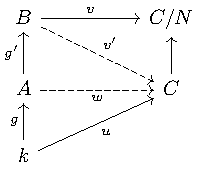
\includegraphics[height=21em]{./figure/ci.pdf}
}

\newcommand{\bookoriginaledition}{1980}
\newcommand{\bookthisedition}{2022}

%these are meant for the back cover
%both should have ~100 words
\newcommand{\bookreview} 
{This book, based on the author's lectures at Brandeis University in 1967 and
1968, is designed for use as a textbook on commutative algebra by students of
modern algebraic geometry or abstract algebra.\\
Part I is devoted to basic concepts such as dimension, depth, normal rings, and
regular local rings; Part II deals with the finer structure theory of noetherian
rings initiated by Zariski and developed by Nagata and Grothendieck.\\
In this second edition, the chapter on Depth has been completely rewritten.
There is also a new Appendix consisting of several sections, which are almost
independent of each other. The Appendix has two purposes: to prove the 
theorems used but not proved in the text; to record same of the recent
achievements in the areas connected with Part II.\\
For specialists in commutative algebra, this book will serve as an introduction
to the more difficult and detailed books of Nagata and Grothendieck.
To geometers, it will be a convenient handbook of algebra. 
}

\newcommand{\bookauthorbio}
{\defemph{Hideyuki Matsumura}\\
Professor of Mathematics at Nagoya University, received his graduate training
at Kyoto University and was awarded his Ph.D. in 1959. Formerly Associate
Professor of Mathematics at this university, Professor Matsumura was a
research associate at the University of Pisa during 1962 and 1963. He was also
Visiting Associate Professor at the University of Chicago (1962), at Johns
Hopkins University (1963), at Columbia University (1966-1967), and at
Brandeis University (1967-1968).\\
The author spent 1973 and 1974 as Visiting Professor at the University of
Pennsylvania, 1974 and 1975 as Visiting Professor at the Politecnic of Torino,
and 1977 as Visiting Professor at the University of Munster. 
}
%\newcommand{\authorbiosource}{insert sources here for the bio/review.} 

%\newcommand{\aboutandlegal}{} %UNUSED -- blurb about what the group is and maybe mention legal stuff in back cover